%PROJECTILE MOTION
\newexp

\section*{Before Lab}

BEFORE COMING TO LAB: Do some preliminary uncertainty analysis.  You
will be calculating the horizontal velocity $v_{x}$ of a
projectile from your measurements
of horizontal distance $x$ and vertical distance $y$, using
Eq.~(\ref{eq:vx}).  Read through the write-up and be sure you
understand the theory, and how the experiment works.

Since these measurements will
have uncertainties $\delta x$ and $\delta y$, there will be a
resulting
uncertainty $\delta v_{x}$ in the calculated velocity.  Work out an
expression for its {\em relative} uncertainty $\delta v_{x}/v_{x}$
in terms of the relative uncertainties of the measurements.  See Appendix
A for help.

 Get your TA to initial your preliminary uncertainty
analysis.


\section*{Introduction}
     Continuing the work of his Medieval predecessors, Richard Swineshead,
William Heytesbury, John Buridan, and John Dumbleton, Galileo was greatly
concerned with the science of motion: how one describes the behavior
of
moving bodies.  One of his particular interests was
projectile
motion. In his work {\em Two New Sciences}, he writes:
\begin{quote}
\begin{center}
On the Motion of Projectiles
\end{center}
We have considered properties existing in equable motion, and those in
naturally accelerated motion over inclined planes of whatever slope.  In
the studies on which I now enter, I shall try to present certain leading
essentials, and to establish them by firm demonstrations, bearing on a
moveable when its motion is compounded from two movements; that is, when it
is moved equably and is also naturally accelerated.  Of this kind appear to
be those which we speak of as projections, the origin of which I lay down
as follows.

I mentally conceive of some moveable projected on a horizontal plane, all
impediments being put aside.  Now it is evident from what has been said
elsewhere at greater length that equable motion on this plane would be
perpetual if the plane were of infinite extent, but if we assume it to be
ended, and [situated] on high, the moveable (which I conceive of as being
endowed with heaviness), driven to the end of this plane and going on
further, adds on to its previous equable and indelible motion that downward
tendency which it has from its own heaviness.  Thus there emerges a certain
motion, compounded from equable horizontal and from naturally accelerated
downward [motion], which I call ``projection."  We shall demonstrate some of
its properties [accidentia], of which the first is this:
\begin{center}
PROPOSITION I.  THEOREM I.
\end{center}
\begin{quote}
When a projectile is carried in motion compounded from equable horizontal
and from naturally accelerated downward [motions], it describes a
semiparabolic line in its movement.
\end{quote}
\end{quote}

Galileo had discovered a fascinating concept: The motion of
an object in the earth's gravity is accelerated downward with the same
acceleration {\em irrespective of its horizontal velocity}.
So if one neglects air resistance, an object dropped from 40 meters will
hit the ground at the same time
as a similar object launched horizontally from the same height.  One
can analyze the vertical motion separately from any horizontal
movement.

The purpose of this experiment is to investigate Galileo's conclusions
about projectile motion:  that it is compounded of two
independent motions---a horizontal component and a vertical
component---and that the path followed is parabolic.
%\section*{Video Lab}
%You and the the rest of the class will become camera jockeys in this lab by filming the
%motion of a projectile.  The TA will be helping you to set up and record
%a projectile flight clearly enough that you can take data from the frame-by-frame
%advance of the film.  This data will have bigger error than the experiment which follows,
%but is a great way for you to quickly see that the trajectory of a launched object is,
%indeed, parabolic.  Show this by fitting your rough $y$ vs $t$ via LINFIT (You can
%use the first half of flight if you wish). This is to be a class project.  In your final
%summary of this data, describe what you saw in the video in the x-direction and
%y-direction independently.  {\em Note: you can use units of Frames for the time
%and Bricks for the distance}

\section*{Experiment}

\begin{figure}[hbt]
\begin{center}
{\resizebox{5in}{!}{{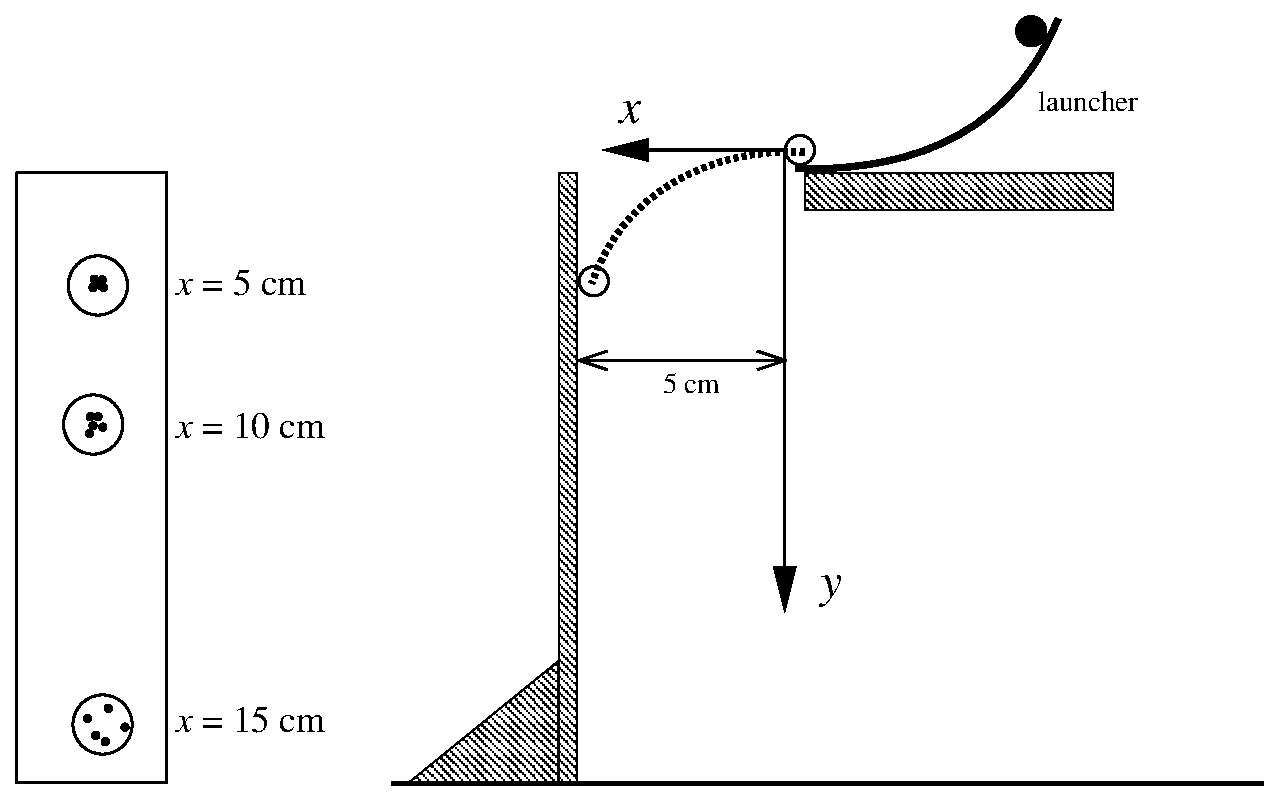
\includegraphics{projectile.app.eps}}}}
\end{center}
%\vspace{3in}
%\special{eps:projectile.app.eps x=5in y=3in}
%\special{wmf:figa1.wmf} % x=3.44in y=1.5in}
 \caption{Projectile motion apparatus.  \label{fig:projectile}}
\end{figure}
The apparatus for this experiment is simple, but can yield reasonably
good data if careful measurements are made.  You will be
launching steel ball bearings as projectiles.  A projectile launcher
will
get the ball moving and launch it horizontally (i.e., $v_{0y}=0$) from a table towards a
vertical board covered with carbon paper.
The carbon paper marks the ball's point of impact.
The horizontal distance $x$ traveled is changed by moving the board
further and further away. The vertical distance $y$ it falls
will be measured as a function of $x$.  The relationship between these distances determines
the shape of the ball's flight path.

The important equations should be familiar by now.  If the projectile has a
constant velocity $v_{x}$ in the $x$ direction, and is gravitationally accelerated in
the $y$ direction, then
\begin{eqnarray}
x & \!\!= &\!\! v_{x}t \\        \label{eq:xproj(t)}
y & \!\!= &\!\! \frac{1}{2}gt^{2} \label{eq:yproj(t)}
\end{eqnarray}
where $t$ is the time for the ball to fall a distance $y$ and move
a distance $x$ horizontally.
From Eq.~(\ref{eq:yproj(t)}) we see that the time of flight is
\begin{equation}
t = \sqrt{\frac{2y}{g}}  \label{eq:t(y)}
\end{equation}
so the horizontal velocity is
\begin{equation}
v_{x} = x/t =  x\sqrt{\frac{g}{2y}} \label{eq:vx}
\end{equation}
If we square both sides and solve for $y$, we obtain
\begin{equation}
y = \frac{g}{2v_{x}^{2}}x^{2}, \label{eq:y(x)}
\end{equation}
which is the equation of a parabola.  You will be testing whether $v_{x}$
does in fact remain constant, and whether the path is parabolic.

\section*{Procedure}
\begin{enumerate}

\item Attach paper to the board.  Use the launcher to make a horizontal line
on the paper representing $y = 0$.

Use a plumb line from the end of the launcher to set the $x = 0$ point on the
floor.  Notice that you will need to correct the horizontal distance $x$ for
the radius of the ball, and the launch position of the ball as it leaves the
launcher.  Check with your instructor if you are uncertain about this correction.  

%Note the inconvenient location of the origin:
%at the far edge of the ball --- a radius up in $y$ and a radius less in $x$ from the track end.
%The easiest solution is to use the track-end as the origin in recording data, and then
%adjust the $(x,y)$ locations all at once in the spreadsheet.  Make a horizontal line on the
%paper representing the height of the track surface and vertical line as an aim point for the
%balls.

\item  Attach carbon paper to the board, so that the ball will leave a mark where
it hits the board. 
Move the board 5 cm away from the end of the launcher (so that your first (uncorrected) 
horizontal distance is $x$ = 5 cm);
Estimate of the
uncertainty, $\delta x$, in the boards location. Use a level to check that the board is vertical. 
Now launch the ball and check that it
left a carbon mark on the paper where it hit the board.  Repeat four more times. 
%{\em Note: Observe all safety precautions in the lab!}

\item  Estimate the vertical distance
the ball traveled for an average trial.  Estimate the uncertainty $\delta y$ from the
half the spread in $y$.

\item  Continue these measurements for horizontal distances of 10, 15,\ldots
50 cm.  Make a table for your data and calculations something like this:

\begin{center}
\begin{tabular}{|c|c|c|c|c|c|}
\hline
$x$ & $\delta x$& $y$ & $\delta y$& $v_{x}$ & $\delta v_{x}$ \\
 (cm) & (cm)   &  (cm)& (cm)      & (cm/s) &  (cm/s)\\
\hline
 \phantom{10000}& \phantom{10000}   &  \phantom{10000}& \phantom{10000}      & \phantom{10000} &  \phantom{10000} \\
\hline
  &   &  &  &  &      \\ \hline
  &   &  &  &  &      \\ \hline
\end{tabular}
\end{center}
\item Calculate the velocities $v_{x}$ for the table.  Their uncertainties
should be easy to compute using the formula you worked out before coming to
lab.  Does $v_{x}$ appear to be constant, within the limits of your uncertainties?

%\item Make a graph of $y$ vs.\ $x$, including error bars to indicate the
%uncertainties, and sketch the curve as best you can.

\item  In this experiment, the errors in both $x$ and $y$ are
typically non-negligible, and so you will probably want to
include the uncertainty in $x$ in your least-squares fit in Linfit.

%Be sure to include the $x$ error bars on your graphs.

%There is a complication in using LINFIT this time.  Because of
%the nature of the numerical algorithm generally used for least-squares
%fits, LINFIT will only accept uncertainties in $y$, and not in $x$.
%But your data probably has significant errors in both $y$ and $x$.
%One way to deal with this problem is to transform the uncertainties in
%$x$ into additional uncertainties in $y$.
%
%Graphically, this scheme is not hard to follow.  Examine your graph of
%$y$ vs. $x$, and note that an uncertainty in $x$---a horizontal error
%bar---has the same effect as a proportionally {\em larger} $y$ error
%bar.  Be sure you understand this point qualitatively.
%
%The mathematics requires a little bit of calculus.  We begin
%by rewriting Eq.~(\ref{eq:y(x)}):
%
%\[
%y = \frac{g}{2v_{x}^{2}}x^{2}
%\]
%
%Next, take the derivative of $y$ with respect to $x$:
%\[
%{dy \over dx} = {g \over {v_{x}^2}} x  = {2y \over x}
%\]
%where the result on the right follows by substitution---take a few
%minutes and be sure you understand how the calculation works.
%
%If we convert this result from a derivative to a differential, we
%obtain
%
%\[
%\delta y = 2y {\delta x \over x}
%\]
%In this form, we have an equation that gives the uncertainty in $y$
%due to a corresponding uncertainty in $x$.  The total uncertainty in
%$y$, then, is this result added to the experimental uncertainty in
%$y$.  If we call this total uncertainty $\delta y'$, we have
%
% \begin{displaymath}
%  \delta y' =  \delta y + 2 y \frac{\delta x}{x}
%\end{displaymath}
%as the uncertainty.  Compute a list of these ``corrected"
%uncertainties to go with your $y$ data.  It may be convenient to
%use a spreadsheet for these calculations.

\item Use LINFIT to test whether $y(x)$ is a parabola; fit the data using
the form $Y = AX^{B}$, where $B$ is not a fixed constant, but a variable to
be determined by LINFIT.  Compare your values for the parameters $A$ and $B$
to the predictions of Eq.~(\ref{eq:y(x)}).  $B$ ought to be somewhere near
2, and $A$ should be approximately $g/(2v_{x}^{2})$.
Make normal and log-log plots of your results.

\item A better value for $A$ is obtained if we fit 
to $Y = AX^{B}$ but keep $B$ constant
at 2.  Due to Linfit limitations, this will require turning off
$x$ errors.  Calculate $v_x$ from this $A$ value.

\section*{Conclusions}

Discuss the results of the experiment:  Is the horizontal component of
velocity constant, within experimental uncertainty?  And are your data
consistent with a parabolic path?  As always, give detailed analysis
of your least-squares fits, including a discussion of the reduced
chi-squared value.

\section*{Critique of Lab}
     Follow the suggestions given in the Introduction to the
Laboratory Manual.




\end{enumerate}
\newpage
%\cleardoublepage
%\begin{center}
% CHECKLIST FOR PROJECTILE LAB \\
%\end{center}
%\bigskip
%\begin{center}
%\begin{tabular}{||l|r||}
%ASPECT CONSIDERED & EVALUATION \\ \hline
%Preliminary uncertainty analysis & \\ \hline
%Video Lab Data and analysis (class project) & \\ \hline
%Summary of observations and findings in Video Lab & \\ \hline
%Table of $y$, $x$ data with uncertainties & \\ \hline
%Calculations of $v_{x}$ with uncertainties, and comments on constancy & \\ %\hline
%Graph of $y(x)$ & \\ \hline
%$\delta y$ values corrected for LINFIT analysis & \\ \hline
%LINFIT analysis of $y(x)$ & \\ \hline
%Comparison of A and B parameters with theoretical values & \\ \hline
%Cleanup & \\ \hline
%\end{tabular}
%\end{center}
%\bigskip
%\bigskip
%Comments:\\
